\chapter{Solvers}
\label{chap:solvers}

\section{Overview}
\label{sec:solver-overview}

\ac{EMTG} contains both a local optimizer and a stochastic global search heuristic. The user may choose to run the local optimizer and the stochastic search heuristic, just the local optimizer, or no optimizer at all and instead evaluate an initial guess with no iterations.

\section{Gradient-Based Solver}
\label{sec:gradient-based-solver}

\ac{EMTG} formulates its optimization problems as \ac{NLP} problems. The optimizer solves a problem of the form:
%
\begin{equation}
\begin{array}{l}
{\text{Minimize }}f\left( {\bf{x}} \right) \\ 
{\text{Subject to:}} \\ 
{{\bf{x}}_{lb}} \le {\bf{x}} \le {{\bf{x}}_{ub}} \\ 
{\bf{c}}\left( {\bf{x}} \right) \le {\bf{0}} \\ 
A{\bf{x}} \le \bf{0} \\ 
\end{array}	
\label{eq:NLP}
\end{equation}
%
where $\mathbf{x}_{lb}$ and $\mathbf{x}_{ub}$ are the lower and upper bounds on the decision vector, $\mathbf{c}\left(\mathbf{x}\right)$ is a vector of nonlinear constraint functions, and $A$ is a matrix describing any linear constraints (\textit{e.g.} time constraints).

Most interplanetary trajectory optimization problems consist of hundreds of variables and tens to hundreds of constraints. Such problems are best solved with a \textit{sparse} \ac{NLP} solver such as \ac{SNOPT} \cite{GillSNOPT}. \ac{SNOPT} uses a sparse \ac{SQP} method and benefits greatly from precise knowledge of the problem Jacobian, \textit{i.e.}, the matrix of partial derivatives of the objective function and constraints with respect to the decision variables. \ac{EMTG} provides analytical expressions for all of the necessary partial derivatives, leading to improved convergence \textit{vs.} using numerically approximated derivatives \cite{BoundedImpulseDerivatives1,BoundedImpulseDerivatives2,EllisonPhD}. \ac{SNOPT}, like all \ac{NLP} solvers, requires an initial guess of the solution and tends to converge to a solution in the neighborhood of that initial guess. The next section discusses EMTG's fully automated method for generating initial guesses.

\ac{EMTG}'s \ac{NLP} solver interface consists of the \texttt{NLP\_interface} abstract base class and the \texttt{NLPoptions} data structure. Individual solvers are addressed via derived classes of \texttt{NLP\_interface}. Currently the only such derived class is \texttt{SNOPT\_interface}. \ac{EMTG} could interface to other \ac{NLP} solvers such as IPOPT, SOS, WORHP, \textit{etc.} if the need arose and if licenses to those solvers were provided.

\section{\ac{MBH}}
\label{sec:MBH}

\subsection{Monotonic Basin Hopping}
\label{subsec:MBH}

\ac{EMTG} has the ability to search for globally optimal solutions and to optimize without an initial guess via the \ac{MBH} stochastic global search heuristic \cite{YamDiLorenzoIzzo2011,RaowulfCoverstonePareto,CoverstoneMicroGA,CoverstoneCarroll2000387,VavrinaHowellGAGALLOP,EnglanderConwayWilliamsEMTG,EnglanderConwayWilliamsEMTGLTConferencePaper,EnglanderPhD,EllisonEnglanderConwaySummer2013,EllisonEnglanderOzimekConwayWinter2014,MBH_ISSFD_2014,VavrinaMGAnDSMs}.

\ac{MBH} \cite{ISI:000165808600005} is an algorithm for searching for the best solutions to problems with many local optima. Many problems, including those described in this work, are structured such that individual locally optimal ``basins'' cluster together, where the distance in the decision space from one local optima to the next in a given cluster may be traversed in a short ``hop.'' A problem may have several such clusters. MBH was originally developed to solve molecular conformation problems in computational chemistry, but has been demonstrated to be effective on various types of interplanetary trajectory problems \cite{YamDiLorenzoIzzo2011,ISI:000288709500009,EnglanderConwayWilliamsEMTGLTConferencePaper, EnglanderPhD, EllisonEnglanderConwaySummer2013,ARRM_Option_C}. Pseudocode for \ac{MBH} is given in Algorithm \ref{alg:MBH}, and a diagram of the \ac{MBH} process on a 1-dimensional function is shown in Figure \ref{fig:MBH}.

Special attention is given to decision variables that define the time-of-flight between two boundary points, \textit{e.g.} Earth or Trojan flybys in Lucy. These are the most significant variables that define at trajectory and therefore it is sometimes necessary to drastically perturb them in order to ``hop'' to a new cluster of solutions. With some (low) uniform-random probability $\rho$, each time-of-flight variables is shifted by $\pm$ 1 synodic period of the two boundary points defining that trajectory phase. In preliminary design for Lucy, $\rho$ was set to 0.05. In high fidelity re-optimization, $\rho$ is set to 0.0, because we do not expect significant changes to the trajectory.

\begin{algorithm}
	\caption{Monotonic Basin Hopping (\acs{MBH})\label{alg:MBH}}
	\begin{algorithmic}
		\State generate random point $\mathbf{x}$
		\State run NLP solver to find point $\mathbf{x}^*$ using initial guess $\mathbf{x}$
		\State $\mathbf{x}_{current} = \mathbf{x}^*$
		\If {$\mathbf{x}^*$ is a feasible point}
		\State save $\mathbf{x}^*$ to archive
		\EndIf
		\While {not hit stop criterion}
		\State generate $\mathbf{x}'$ by randomly perturbing $\mathbf{x}_{current}$
		\For {each time-of-flight variable $t_i$ in $\mathbf{x}'$}
		\If {$rand\left(0,1\right) < \rho_{time-hop}$}
		\State shift $t_i$ forward or backward one synodic period
		\EndIf
		\EndFor
		\State run NLP solver to find locally optimal point $\mathbf{x}^*$ using in initial guess $\mathbf{x}'$
		\If {$\mathbf{x}^*$ is feasible \textbf{and} $f\left(\mathbf{x}^*\right) < f\left(\mathbf{x}_{current}\right)$}
		\State $\mathbf{x}_{current} = \mathbf{x}^*$
		\State save $\mathbf{x}^*$ to archive
		\Else { \textbf{if} $\mathbf{x}^*$ is infeasible \textbf{and} $\left\|c\left(\mathbf{x}^*\right)\right\| < \left\|c\left(\mathbf{x}_{current}\right)\right\|)$}
		\State $\mathbf{x}_{current} = \mathbf{x}^*$
		\EndIf
		\EndWhile	\\			
		\Return best $\mathbf{x}^*$ in archive
	\end{algorithmic}
\end{algorithm}

\begin{figure}
	\centering
	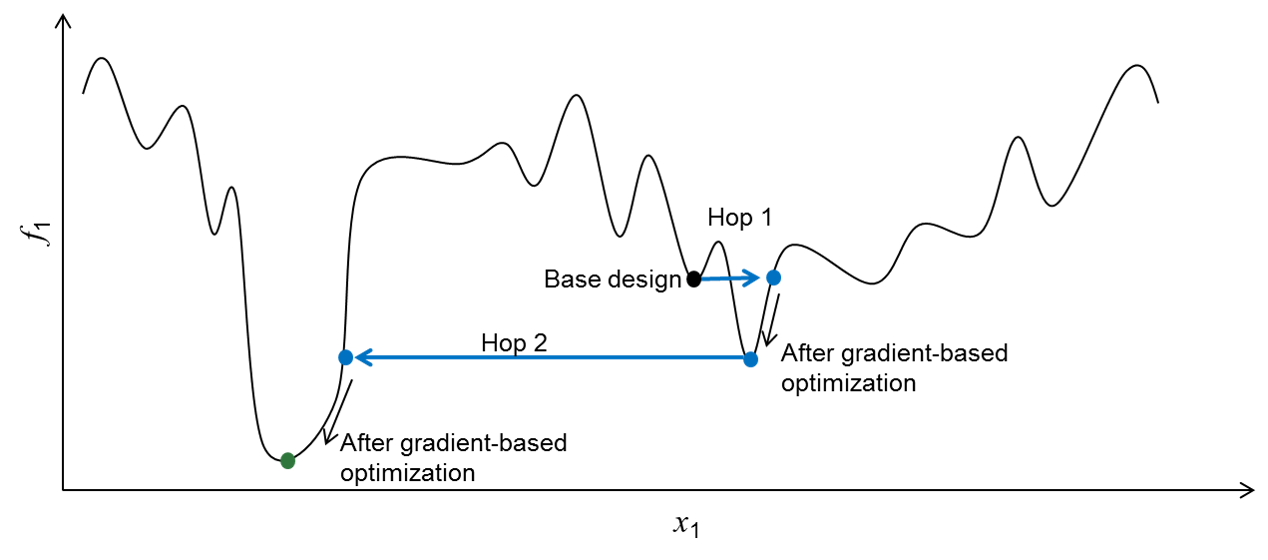
\includegraphics[width=0.8\linewidth]{MBH.png}
	\caption{ Monotonic Basin Hopping on a 1-dimensional function.}
	\label{fig:MBH}
\end{figure}

\ac{MBH} is run until either a specified number of iterations (trial points attempted) or a maximum CPU time is reached, at which point the best solution stored in the archive is returned. The version of \ac{MBH} used in EMTG has two parameters: the stopping criterion and the type of random step used to generate the perturbed decision vector $\mathbf{x}'$. In this work, the random step is drawn from a bi-directional Pareto distribution with the Pareto parameter, $\alpha$, set to 1.4. The bi-directional Pareto distribution usually generates small steps that allow \ac{MBH} to \textit{exploit} the local cluster around the current best solution. However, some of the steps generated by the bi-directional Pareto distribution are much larger, in some cases spanning the entire decision space. These larger steps allow \ac{MBH} to \textit{explore} the full decision space. This approach has been shown to be robust on complex interplanetary trajectory design problems \cite{MBH_ISSFD_2014}.

\ac{MBH} may be started either from a uniform-randomly chosen point in the decision space or from an initial guess derived from a previous problem. As long as the two problems are sufficiently similar, the latter approach is more efficient than starting from randomness. However, on simple problems, \ac{MBH} will quickly find the global best solution with or without an initial guess.

\section{Initial Guess}
\label{sec:initial_guess}

If the user chooses to specify an initial guess to \ac{MBH} or to run \ac{EMTG} in \ac{NLP}-only or evaluate-only mode, then an initial guess must be provided. \ac{EMTG} features an intelligent initial guess parser that is designed to minimize load on the user. This process is actually executed by the \texttt{Mission} class but is described here because this is where users would expect to find it. The initial guess parser obeys the following rules:

\begin{enumerate}
	\item The initial guess is specified at the Journey level, in the \texttt{trialX} field of each \texttt{JourneyOptions} object. The user may type or paste the initial guess into the corresponding \texttt{trialX} field for each journey in the .emtgopt input script.
	\item Each entry in the initial guess is a comma-separated tuple. The first element is the name of the decision variable and the second element is the value. The name of each decision variable can be found by running \ac{EMTG} with no initial guess and reading the resulting XFfile.csv that lists all decision variables and constraints.
	\item While \ac{EMTG}'s internal time calculations are performed in seconds, we recognize that humans like to think in days and so time variables in the initial guess are parsed in days.
	\item If any decision variable is \textit{not} specified, \ac{EMTG} will assign a uniform random number between the bounds of that variable. It is therefore possible to supply a partial initial guess. \ac{EMTG} warns the user when it does this.
	\item Decision variables related to a number of time steps, such as control variables in a \texttt{TwoPointShootingPhase} or state and control variables in a \texttt{ParallelShootingPhase} are interpolated to the number of time steps present in the phase. The user may specify an initial guess with a different number of time steps than the mission is configured for - \ac{EMTG} will figure it out.
	\item Decision variables in the initial guess whose names are not recognized are ignored.
\end{enumerate}